\chapter{几何光学：光线、反射与折射}\label{ch:b1:rays-reflection-refraction}

插在水杯里的吸管，在水面处看上去像是折断了；
从池底仰望的游泳者，看到整片天空被挤压成
一个明亮的圆盘，圆盘周围环绕着池底的镜像；一根细如发丝的玻璃纤维，
能把一通电话跨越大洋传送，其损耗比
铜线跨越一条街道时还要小。三条定律——光
沿直线传播、等角反射、依斯涅耳定律折射——足以
解释上述一切。本章将准确陈述它们，指出它们在何处不再成立，
并将其付诸应用。

\begin{omfigure}
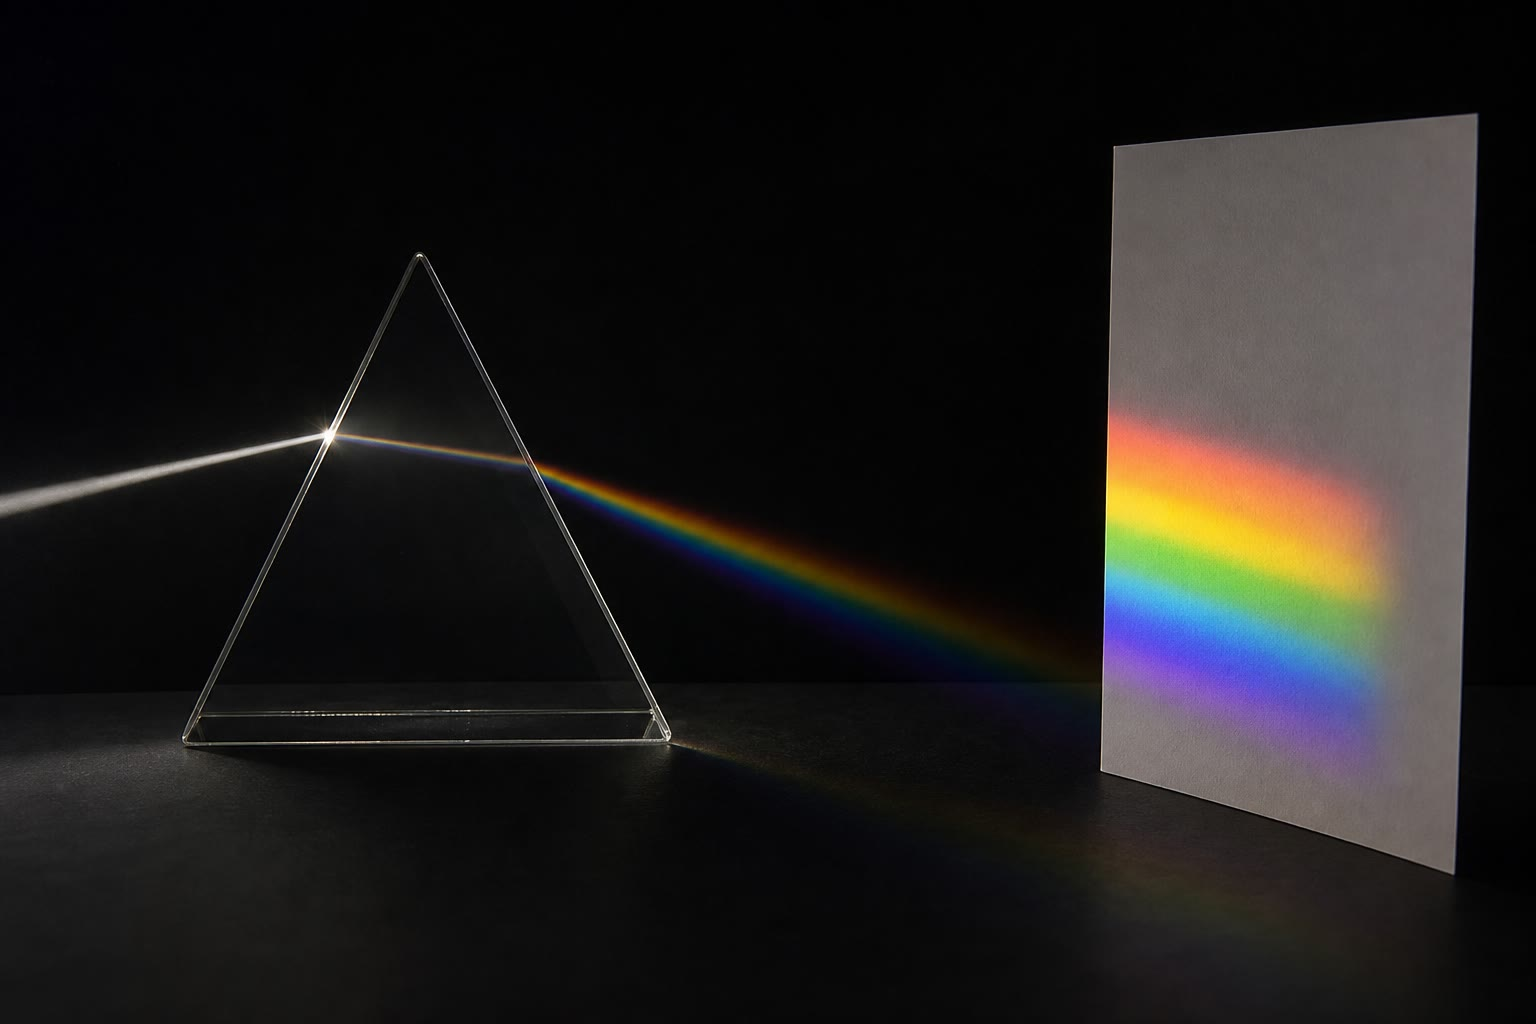
\includegraphics[width=0.58\linewidth]{images/book3/ai/b3-02-prism-dispersion-v2.jpg}

{\small 棱镜使白光束向其底边偏折，并使之色散：玻璃的折射率依赖于波长，紫光偏折最大。}
\end{omfigure}

\section{几何光学模型}

\begin{definition}[光线；均匀介质]\label{def:b1:rays-reflection-refraction:ray}
\index{光线}\index{几何光学}\index{均匀介质}
在\emph{几何光学}模型中，光沿
\emph{光线}传播。光线是带方向的曲线，在
\emph{均匀}介质（各点性质相同）中为直线，且
彼此独立地携带能量。光束是光线的集合；
点光源向各个方向发出光线。
\end{definition}

\begin{definition}[折射率]\label{def:b1:rays-reflection-refraction:index}
\index{折射率}\index{透明介质}
\emph{透明}介质允许光通过；光在其中以
速率 $v < c$ 传播。其\emph{折射率}为
\[
n = \frac{c}{v} \geq 1 .
\]
真空：$n = 1$；空气：$1.0003$；水：$1.33$；普通玻璃：$1.5$
至 $1.6$；金刚石：$2.42$。频率为 $\nu$ 的波进入介质后
其频率保持不变，波长由真空中的 $\lambda_0 =
c/\nu$ 减小为 $\lambda = \lambda_0/n$。
\end{definition}

\begin{remark}[色散]\label{rem:b1:rays-reflection-refraction:dispersion}
\index{色散（光学）}\index{柯西经验公式}
在物质中，折射率略依赖于波长——介质是
\emph{色散的}。对于可见光波段的玻璃，柯西经验公式
$n(\lambda) = A + B/\lambda^2$ 拟合得很好：蓝光对应的 $n$ 比红光的
大约大 $0.01$ 至 $0.02$。本章末尾的棱镜与彩虹，
正是建立在这一差异之上。
\end{remark}

\begin{remark}[模型的局限]\label{rem:b1:rays-reflection-refraction:limits}
光是一种波，波穿过宽度为 $a$ 的孔时
会以量级为 $\lambda/a$ 的角度展开（衍射，
见\cref{ch:b1:wave-propagation}）。只要每个孔径、透镜和障碍物
都远大于波长，光线描述就是适用的，
（可见光的波长为 \qty{0.4}{} 至 \qty{0.8}{\micro m}）：一个 \qty{1}{mm}
的小孔使光束展开 $10^{-3}$ 弧度，在实验台上可忽略不计；一个
\qty{1}{\micro m} 的孔则使光束扩展到整个半空间，光线图像便不再成立。
单模电信光纤的 \qty{9}{\micro m} 纤芯
已超出该模型的适用范围。
\end{remark}

\begin{proposition}[光路可逆]\label{prop:b1:rays-reflection-refraction:reversibility}
\index{光路可逆原理}
光线所经的路径不依赖于光沿其传播的方向：
若光沿某条路径从 $A$ 到达 $B$，则从 $B$ 出发的光
会沿同一路径回到 $A$。
\end{proposition}
\admitted

\section{反射与折射}

\begin{definition}[入射]\label{def:b1:rays-reflection-refraction:incidence}
\index{入射面}\index{入射角}\index{折射面}
一条光线射到分隔两种介质的界面（即\emph{折射面}）上的
点 $I$ 处，与界面在 $I$ 处的\emph{法线}所成的
角为\emph{入射角} $i_1$。\emph{入射面}包含
入射光线与法线。
\end{definition}

\begin{theorem}[反射与折射定律（斯涅耳–笛卡儿）]\label{thm:b1:rays-reflection-refraction:snell}
\index{反射!定律}\index{折射!定律}\index{斯涅耳定律}
在折射率分别为 $n_1$（入射侧）与
$n_2$ 的两种介质的界面上：
\begin{enumerate}
  \item 反射光线与折射光线位于入射面内；
  \item 反射光线与法线所成的角为 $i_1' = i_1$，
        位于法线的另一侧；
  \item 折射光线与法线所成的角 $i_2$ 满足
        \[
        n_1 \sin i_1 = n_2 \sin i_2 .
        \]
\end{enumerate}
\end{theorem}
\admitted

\begin{remark}[定律的来源]\label{rem:b1:rays-reflection-refraction:fermat}
\index{费马原理}
两条定律均可由\emph{费马原理}导出：光在两点之间
沿传播时间最短的路径前进。等角反射是
经过镜面的最短折线路径；斯涅耳定律则是
在快介质中多走一段、在慢介质中少走一段的路径，
两者之间的权衡（见\cref{exo:b1:rays-reflection-refraction:12}）。
在本科二年级分册中，两条定律均由光在界面处的
波动本质推导得出。
\end{remark}

\begin{omfigure}
\begin{tikzpicture}[font=\small, x=1cm, y=1cm]
  \fill[omDef!10] (-3.6,-2.4) rectangle (3.6,0);
  \draw[thick] (-3.6,0) -- (3.6,0);
  \draw[dashed] (0,-2.4) -- (0,2.6) node[above] {法线};
  \node at (-3.0,0.4) {$n_1$};
  \node at (-2.85,-0.45) {$n_2 > n_1$};
  % incident at 50 deg from normal
  \draw[-Stealth, omThm, thick] (-2.3,1.93) -- (-1.15,0.965);
  \draw[omThm, thick] (-1.15,0.965) -- (0,0);
  % reflected
  \draw[omThm, thick] (0,0) -- (1.15,0.965);
  \draw[-Stealth, omThm, thick] (1.15,0.965) -- (2.3,1.93);
  % refracted at 31 deg
  \draw[omDef, thick] (0,0) -- (0.62,-1.03);
  \draw[-Stealth, omDef, thick] (0.62,-1.03) -- (1.24,-2.06);
  \draw (0,1.1) arc (90:140:1.1); \node at (-0.5,1.4) {$i_1$};
  \draw (0,1.1) arc (90:40:1.1); \node at (0.5,1.4) {$i_1'$};
  \draw (0,-1.1) arc (270:301:1.1); \node at (0.45,-1.45) {$i_2$};
  \fill (0,0) circle (1.2pt); \node[above left, xshift=-2pt] at (0,0) {$I$};
\end{tikzpicture}

{\small 两种介质分界面上的反射与折射。
当 $n_2 > n_1$ 时折射光线向法线偏折；三条光线
与法线同处一个平面，即图所在的平面。}
\end{omfigure}

\begin{proposition}[光线的弯折方向]\label{prop:b1:rays-reflection-refraction:bending}
光线进入折射率较大的介质（$n_2 > n_1$）时，
会\emph{靠近}法线（$i_2 < i_1$）；进入折射率较小的介质时，
则\emph{远离}法线（$i_2 > i_1$）。沿法线入射的光线
不发生偏折。
\end{proposition}

\begin{proof}
$\sin i_2 = (n_1/n_2)\sin i_1$，其中 $\sin$ 在
$[0, \pi/2]$ 上递增。
\end{proof}

\begin{example}[视深]\label{ex:b1:rays-reflection-refraction:depth}
\index{视深}
一枚硬币位于水下深 $h$ 处（$n = 1.33$），从几乎正上方
观察。硬币发出的光线以小角度 $i_2$（在水中）到达水面，
以 $i_1$ 射出，且 $\sin i_1 = n\sin i_2$；小角度时
$i_1 \approx n\,i_2$。人眼将出射光线反向延长，
认为它来自深度为 $h'$ 处，且 $\tan i_1 \approx x/h'$ 与
$\tan i_2 \approx x/h$ 成立（$x$ 为同一水面点到竖直线的距离），
于是 $h' = h\,i_2/i_1 = h/n$。一个深 \qty{2.0}{m} 的水池看起来
只有 \qty{1.5}{m} 深；鱼看见钓鱼的人，
比他实际高出 $1.33$ 倍。
\end{example}

\begin{theorem}[全反射]\label{thm:b1:rays-reflection-refraction:tir}
\index{全反射}\index{临界角}
光由折射率为 $n_1$ 的介质射向折射率较小的介质
（$n_2 < n_1$）时，仅当 $i_1 \leq i_c$ 才发生折射，其中
\emph{临界角}满足
\[
\sin i_c = \frac{n_2}{n_1} .
\]
当 $i_1 > i_c$ 时不存在折射光线，界面将
全部光线反射——即\emph{全反射}。
\end{theorem}

\begin{proof}
由斯涅耳定律得 $\sin i_2 = (n_1/n_2)\sin i_1 > \sin i_1$，
此式超过 $1$（即 $\sin i_1 > n_2/n_1$）时，
便不存在与之对应的角 $i_2$。当 $i_1 = i_c$ 时，折射光线掠过界面
（$i_2 = 90^\circ$）。此时能量\emph{全部}被反射，这是关于
光强的论断，几何光学不予处理；
本科二年级分册中的波动处理对此予以证实。
\end{proof}

\begin{omfigure}
\begin{tikzpicture}[font=\small, x=1cm, y=1cm]
  \fill[omDef!10] (-4.2,-2.2) rectangle (4.2,0);
  \draw[thick] (-4.2,0) -- (4.2,0);
  \node at (3.0,0.85) {空气 $n_2 = 1$};
  \node at (2.9,-0.55) {水 $n_1 = 1.33$};
  \fill (-3,-2) circle (1.5pt) node[below] {$S$};
  % ray 1: i1 = 30 deg -> hits surface at x = -3 + 2 tan30 = -1.845 ; refracted i2 = 41.7
  \draw[-Stealth, omThm, thick] (-3,-2) -- (-1.845,0);
  \draw[-Stealth, omThm, thick] (-1.845,0) -- ++(41.7:1.6);
  % ray 2: i1 = 48.8 (critical): hits at x = -3 + 2 tan48.8 = -0.716 ; refracted grazing
  \draw[-Stealth, omProp, thick] (-3,-2) -- (-0.716,0);
  \draw[-Stealth, omProp, thick] (-0.716,0) -- (1.3,0.02);
  \draw[omProp, thick] (-0.716,0) -- ++(131.2:1.5);
  % ray 3: i1 = 65: hits at x = -3 + 2 tan65 = 1.289 ; totally reflected
  \draw[-Stealth, omDef!70!black, thick] (-3,-2) -- (1.289,0);
  \draw[-Stealth, omDef!70!black, thick] (1.289,0) -- ++(115:2.1);
  \draw[dashed] (-1.845,-1.0) -- (-1.845,1.0);
  \draw (-1.845,-0.6) arc (270:240:0.6); \node at (-2.2,-0.85) {$i_1$};
  \node[omThm] at (-1.55,1.35) {\footnotesize 折射};
  \node[omProp, right] at (1.45,0.3) {\footnotesize 掠射，$i_1 = i_c$};
  \node[omDef!70!black] at (1.55,2.05) {\footnotesize 仅反射};
\end{tikzpicture}

{\small 水下光源 $S$ 发出的光线。低于临界角
（水–空气界面的 $i_c = 48.8^\circ$）时，部分光线射出；在 $i_c$
处折射光线掠过界面；超过此角度后，界面成为
理想镜面——游泳者看到的明亮天空圆盘，其边界由该角度决定。}
\end{omfigure}

\begin{example}[钻石与游泳者]\label{ex:b1:rays-reflection-refraction:tir}
玻璃–空气：$\sin i_c = 1/1.5$，$i_c = 41.8^\circ$，这就是为何
$45^\circ$ 棱镜能发生全反射，从而在双筒望远镜中代替镜子。
钻石–空气：$i_c = 24.4^\circ$；切割后的钻石会将从
顶面射入的光线困在其中，并几乎全部从顶面射出——
“亮度”来自全反射，“火彩”来自色散。水–空气：
$i_c = 48.8^\circ$；仰望时，潜水者看到的整个天空位于
半顶角为 $48.8^\circ$ 的圆锥内（“斯涅耳窗”），圆锥外则看到
池底的反射。
\end{example}

\section{光纤}

\begin{definition}[阶跃折射率光纤]\label{def:b1:rays-reflection-refraction:fiber}
\index{光纤}\index{纤芯}\index{包层}\index{数值孔径}
\emph{阶跃折射率光纤}由圆柱形玻璃\emph{纤芯}构成，纤芯折射率为
$n_1$，外包着折射率略低、为 $n_2$ 的\emph{包层}。
射入纤芯、且位于以轴为中心、半顶角为 $\theta_a$ 的圆锥内的光线，
将在纤芯–包层界面上经相继的全反射而被导引。
\emph{数值孔径}为
$\mathrm{NA} = \sin\theta_a$.
\end{definition}

\begin{proposition}[接收锥与模间色散]\label{prop:b1:rays-reflection-refraction:fiber}
\index{接收角}\index{模间色散}
对于入射端面位于空气中的光纤，
\[
\sin\theta_a = \sqrt{n_1^2 - n_2^2} .
\]
在长度为 $L$ 的光纤中，沿轴线传播的导引光线与
最陡的导引光线到达终点时存在如下延迟
\[
\Delta t = \frac{L\,n_1}{c}\left(\frac{n_1}{n_2} - 1\right)
\]
两者之间的延迟即\emph{模间色散}。
\end{proposition}

\begin{proof}
与轴线成 $\theta$ 角入射的光线折射后为 $\theta'$，
满足 $\sin\theta = n_1\sin\theta'$，并以入射角
$i = 90^\circ - \theta'$ 射到包层。导引要求 $\sin i \geq n_2/n_1$，
即 $\cos\theta' \geq n_2/n_1$，亦即 $\sin\theta' \leq
\sqrt{1 - n_2^2/n_1^2}$；两边乘以 $n_1$。沿轴线的光线走过 $L$，
速率为 $c/n_1$，所需时间为 $t_0 = Ln_1/c$。最陡的光线以角度
$\theta'_{\max}$ 之字形前进，$\cos\theta'_{\max} = n_2/n_1$；其路径长为
$L/\cos\theta'_{\max} = L n_1/n_2$，故 $t_1 = L n_1^2/(n_2 c)$，于是
$\Delta t = t_1 - t_0$。
\end{proof}

\begin{omfigure}
\begin{tikzpicture}[font=\small, x=1cm, y=1cm]
  \fill[omDef!6] (0,-1.0) rectangle (7.8,1.0);
  \fill[omDef!18] (0,-0.55) rectangle (7.8,0.55);
  \draw (0,0.55) -- (7.8,0.55); \draw (0,-0.55) -- (7.8,-0.55);
  \draw (0,1.0) -- (7.8,1.0); \draw (0,-1.0) -- (7.8,-1.0);
  \draw[thick] (0,-1.0) -- (0,1.0);
  \draw[dashed] (-0.2,0) -- (7.8,0);
  \node[right] at (7.8,0.78) {包层 $n_2$};
  \node[right] at (7.8,0) {纤芯 $n_1$};
  \node[right] at (7.8,-0.78) {包层 $n_2$};
  % entering ray at theta_a = 25 deg for drawing, refracted to 16 deg
  \draw[-Stealth, omThm, thick] (-1.6,-0.746) -- (0,0);
  \draw[omThm, thick] (0,0) -- (1.92,0.55) -- (5.76,-0.55) -- (7.8,0.035);
  \draw[-Stealth, omThm, thick] (7.0,-0.194) -- (7.8,0.035);
  \draw[dashed] (1.92,1.3) -- (1.92,-0.2);
  \draw (1.92,0.55) ++(0,0.5) arc (90:164:0.5); \node at (1.45,1.2) {$i$};
  \draw[omThm!50, dashed] (-1.6,0.746) -- (0,0);
  \draw (-0.9,0) arc (180:205:0.9); \node at (-1.25,-0.28) {$\theta_a$};
  \draw[omDef!70!black, thick] (0,0) -- (7.8,0);
  \draw (0.9,0) arc (0:16:0.9); \node at (1.2,0.15) {$\theta'$};
  \node[omDef!70!black, below] at (4.0,-1.05) {沿轴光线：路径最短，最先到达};
\end{tikzpicture}

{\small 阶跃折射率光纤。进入半角为 $\theta_a$ 的接收锥内的光线
在包层处的入射角 $i \geq i_c$，借助全反射被导引；
沿轴光线路径最短，最陡的导引光线路径最长，
脉冲在时间上展宽。}
\end{omfigure}

\begin{example}[通信光纤的数值]\label{ex:b1:rays-reflection-refraction:fibernum}
$n_1 = 1.480$，$n_2 = 1.465$：$\mathrm{NA} = \sqrt{2.190 - 2.146} =
0.21$，$\theta_a = 12^\circ$；$i_c = 81.8^\circ$，故导引光线
与轴线夹角在 $8.2^\circ$ 以内。模间展宽：$\Delta t/L =
(1.48/c)(1.48/1.465 - 1) = \qty{51}{ns/km}$。经 \qty{2}{km} 光纤后，脉冲
展宽 \qty{0.1}{\micro s}，这将比特率限制在约
\qty{5}{Mbit/s}：周末问题沿着这一限制，引出其补救办法——
即单模光纤。
\end{example}

\section{平面镜}

\begin{proposition}[平面镜成像]\label{prop:b1:rays-reflection-refraction:mirror}
\index{平面镜}\index{虚像}\index{严格成像}
从点 $A$ 出发、经平面镜反射的所有光线，看似都来自
点 $A'$，它与 $A$ 关于镜面所在平面对称；$A'$
即 $A$ 的\emph{像}。它是\emph{虚像}（没有光线真正经过它），
平面镜是\emph{严格成像}的：每一点都有
精确的点像。
\end{proposition}

\begin{proof}
从 $A$ 射向镜面上点 $I$、入射角为 $i$ 的光线，以
与法线另一侧成 $i$ 角射出。反射线与
点 $I$ 处的法线夹角为 $i$，直线 $IA$ 同样如此；由关于镜面的对称性，
反射线即直线 $IA$ 关于镜面的对称像，
因而经过对称点 $A'$ ——对每一个
$I$ 均成立。
\end{proof}

\begin{proposition}[转动平面镜]\label{prop:b1:rays-reflection-refraction:rotation}
将平面镜绕其所在平面内的一根轴转过角度 $\alpha$，
该轴与入射面垂直，此时反射光线转过的角度为
$2\alpha$。
\end{proposition}

\begin{proof}
法线转过 $\alpha$，故入射角由 $i$ 变为
$i + \alpha$；反射光线位于新法线另一侧，与之成 $i + \alpha$ 角，
相对原方向转过的角为 $\alpha$（法线）$+ \alpha$（角度）$=
2\alpha$。
\end{proof}

\begin{example}[检流计的杠杆]\label{ex:b1:rays-reflection-refraction:galvanometer}
一面小镜子粘在检流计线圈上，由灯照亮，并在
相距 \qty{2}{m} 的标尺上投出光斑：线圈转过
$\qty{1}{mrad}$ 时，光斑移动 $2 \times 10^{-3} \times
\qty{2}{m} = \qty{4}{mm}$ ——一种无摩擦的光学杠杆，能够放大微小转动，
其原理即镜式检流计与激光
扫描仪的原理。
\end{example}

\section{棱镜}

\begin{proposition}[棱镜公式]\label{prop:b1:rays-reflection-refraction:prism}
\index{棱镜}\index{偏向角}\index{最小偏向角}
光线在空气中穿过顶角为 $A$、折射率为 $n$ 的棱镜，
在与棱边垂直的平面内，以法线为基准度量的角 $i$（入射）、$r$、$r'$
（棱镜内）及 $i'$（出射）满足
\[
\sin i = n \sin r, \qquad r + r' = A, \qquad \sin i' = n \sin r',
\]
光线的偏向角为 $D = i + i' - A$。偏向角取最小值的条件是光路
对称，即 $i = i'$，$r = r' = A/2$，此时
\[
n = \frac{\sin\frac{A + D_{\min}}{2}}{\sin\frac{A}{2}} .
\]
\end{proposition}

\begin{proof}
由各折射面上的斯涅耳定律，$r + r' = A$ 是因为两条法线的夹角为
$A$（由顶点、两个入射点与两法线交点构成的四边形），
总偏向角为
$(i - r) + (i' - r') = i + i' - A$。由光路可逆，
偏向角是 $i$ 与 $i'$ 的同一函数；若极小值出现在 $i_0 \neq i_0'$ 处，
则它也会出现在反向入射角
$i_0'$ 处，从而有两个极小值，
这与 $D(i)$ 在其极小值两侧单调的性质相矛盾，故极小值位于 $i = i'$。
于是 $r = r' = A/2$，$D_{\min} = 2i - A$；将 $i = (A +
D_{\min})/2$ 代入 $\sin i = n\sin(A/2)$，即得公式。
\end{proof}

\begin{omfigure}
\begin{tikzpicture}[font=\small, x=1cm, y=1cm]
  % prism apex at top, A = 60 deg
  \coordinate (S) at (0,3.2); \coordinate (B1) at (-1.85,0); \coordinate (B2) at (1.85,0);
  \fill[omDef!10] (S) -- (B1) -- (B2) -- cycle;
  \draw[thick] (S) -- (B1) -- (B2) -- cycle;
  \node[above] at (S) {$A$};
  % entry point on left face at height 1.4: left face from (0,3.2) to (-1.85,0); param t: point = S + t*(B1-S)
  \coordinate (I) at (-1.04,1.4);
  \coordinate (J) at (1.04,1.4);
  % normals: left face direction (-1.85,-3.2) normalized; outward normal for left face points to (-3.2,1.85)/3.7 = (-0.865,0.5)
  \draw[dashed] ($(I)+(-0.865*1.3,0.5*1.3)$) -- ($(I)+(0.865*1.2,-0.5*1.2)$);
  \draw[dashed] ($(J)+(0.865*1.3,0.5*1.3)$) -- ($(J)+(-0.865*1.2,-0.5*1.2)$);
  % incident ray at i=49 deg from normal (min deviation for n=1.5, A=60: i=48.6): direction into prism
  % normal into prism at I: (0.865,-0.5), angle -30 deg. Incident direction = rotate by +48.6 -> angle 18.6 deg
  \draw[-Stealth, omThm, thick] ($(I)+(198.6:2.4)$) -- (I);
  \draw[omThm, thick] (I) -- (J);
  \draw[-Stealth, omThm, thick] (J) -- ($(J)+(-18.6:2.4)$);
  \draw[omExo, dashed] (I) -- ($(I)+(18.6:3.9)$);
  % angles
  \node at (-1.94,1.49) {$i$};
  \node at (-0.32,1.19) {$r$};
  \node at (0.32,1.19) {$r'$};
  \node at (1.94,1.49) {$i'$};
  \coordinate (X) at (0,1.75);
  \draw[omExo] ($(X)+(18.6:2.6)$) arc (18.6:-18.6:2.6);
  \node[omExo] at (2.9,1.75) {$D$};
\end{tikzpicture}

{\small 一束光线穿过顶角为 $A$ 的棱镜，入射时向底边方向折射，
出射时再次折射，于是相对原方向（虚线）偏转了 $D = i + i' - A$ 的角度。
在最小偏向角处作图，此时
光路对称。}
\end{omfigure}

\begin{example}[测量折射率]\label{ex:b1:rays-reflection-refraction:prismnum}
将一个 $60^\circ$ 棱镜转动，使黄色光束的偏向角
最小，此时 $D_{\min} = 38.9^\circ$。于是 $n = \sin 49.45^\circ/\sin 30^\circ
= 0.760/0.500 = 1.52$。最小偏向角是测量玻璃折射率的标准方法——
尖锐的极小值通过来回转动棱镜找到，
对微小的装配误差不敏感。
\end{example}

\begin{remark}[薄棱镜与分光镜]\label{rem:b1:rays-reflection-refraction:thin}
当 $A$ 与入射角都很小时，正弦等于对应的角度，
$D \approx (n - 1)A$，与 $i$ 无关：薄棱镜使每条光线偏折同样的角度——
一块玻璃楔就是能使光线弯折的“棱镜”，
而透镜可以看作由许多这样的楔堆叠而成。由于
$n$ 依赖于 $\lambda$，偏向角也随之变化：棱镜把白光散开成光谱
（蓝光偏折最大），这正是
棱镜分光镜的核心。
\end{remark}

\section{彩虹}

\begin{example}[笛卡儿的彩虹]\label{ex:b1:rays-reflection-refraction:rainbow}
\index{彩虹}
一束阳光射入球形雨滴，入射角为 $i$，
经折射（$\sin i = n\sin r$）后在背面反射一次，
再经一次折射射出。每次折射使光线偏转
$i - r$，内反射使其偏转 $\pi - 2r$：总偏转角
为 $D(i) = \pi + 2i - 4r$。对每个 $i$，雨滴中都有光线射入；观察者
看到最亮的光，恰在大量光线几乎沿同一方向射出之处，
即 $D$ 取驻值之处：$\dd D/\dd i = 2 - 4\,\dd r/\dd i
= 0$。对斯涅耳定律求导得 $\cos i = n\cos r\,\dd r/\dd i$，于是
条件化为 $2\cos i = n\cos r$；两边平方并利用
$n^2\cos^2 r = n^2 - \sin^2 i = n^2 - 1 + \cos^2 i$，得
\[
\cos^2 i = \frac{n^2 - 1}{3} .
\]
对水，$n = 1.333$：$i = 59.4^\circ$，$r = 40.2^\circ$，
$D_{\min} = 137.9^\circ$。光线朝太阳一侧返回，
与反太阳方向的夹角为 $180^\circ - 137.9^\circ = 42^\circ$：
彩虹是半顶角为 $42^\circ$ 的圆锥面，围绕
观察者头部的影子。红光（$n = 1.331$）位于 $42.4^\circ$，紫光
（$n = 1.343$）位于 $40.6^\circ$——红光在外，紫光在内。
\end{example}

\begin{omfigure}
\begin{tikzpicture}[font=\small, x=1cm, y=1cm]
  \draw[omDef, thick, fill=omDef!10] (0,0) circle (1.8);
  \coordinate (P) at (-0.916,1.549);
  \coordinate (Q) at (21.0:1.8);
  \coordinate (R) at (-78.6:1.8);
  \coordinate (X) at (4.02,1.549);
  \draw[-Stealth, omThm, thick] (-4.0,1.549) -- (-2.3,1.549);
  \draw[omThm, thick] (-2.3,1.549) -- (P);
  \draw[omThm, thick] (P) -- (Q) -- (R);
  \draw[omThm, thick] (R) -- ($(R)+(-137.9:1.5)$);
  \draw[-Stealth, omThm, thick] ($(R)+(-137.9:1.5)$) -- ($(R)+(-137.9:2.6)$);
  \draw[dashed, omExo] (P) -- (X);
  \draw[dashed, omExo] (R) -- (X);
  \draw[omExo] ($(X)+(0:0.9)$) arc (0:-137.9:0.9);
  \node[omExo] at (4.55,0.45) {$D$};
  \draw[dashed] (P) -- (0,0); \draw[dashed] (Q) -- (0,0); \draw[dashed] (R) -- (0,0);
  \draw[dashed] (P) -- ($(P)+(120.6:0.8)$);
  \draw[dashed] (R) -- ($(R)+(-78.6:0.8)$);
  \node at (-1.57,1.95) {$i$};
  \node at (-0.37,1.11) {$r$};
  \node at (1.08,0.66) {$r$};
  \node at (1.25,0.22) {$r$};
  \node at (0.45,-1.15) {$r$};
  \node at (0.1,-2.45) {$i$};
  \fill (0,0) circle (1pt); \node[above left] at (0,0) {$O$};
  \node[omDef!60!black] at (1.5,2.3) {雨滴，$n = 1.333$};
\end{tikzpicture}

{\small 笛卡儿光线穿过雨滴：两次折射和一次
内反射。在 $i = 59^\circ$ 附近，偏向角 $D$
取驻值 $138^\circ$，光线在此处聚集，形成主彩虹，
位于距对日点 $42^\circ$ 处。}
\end{omfigure}

\section{练习}

\begin{exercise}[$\star$]\label{exo:b1:rays-reflection-refraction:1}
求光在水中（$n = 1.33$）、玻璃中（$1.50$）和
金刚石中（$2.42$）的速率。光穿过
\qty{1.0}{km} 长、折射率为 $1.48$ 的光纤需要多长时间？
\end{exercise}

\begin{exercise}[$\star$]\label{exo:b1:rays-reflection-refraction:2}
一束光线由空气射向水面（$n = 1.33$），入射角为 $30^\circ$，
再为 $60^\circ$（均自法线量起），求各折射角。一束光线在水中
以 $50^\circ$ 的入射角射到水面，会发生什么？
\end{exercise}

\begin{exercise}[$\star$]\label{exo:b1:rays-reflection-refraction:3}
求玻璃–空气（$n = 1.50$）、金刚石–空气
（$2.42$）和水–空气（$1.33$）的临界角。潜水员看到的
天空圆盘的角直径为多少？
\end{exercise}

\begin{exercise}[$\star$]\label{exo:b1:rays-reflection-refraction:4}
一人身高 \qty{1.70}{m}，双眼位于头顶以下 \qty{10}{cm}
处，站在竖直挂于墙上的平面镜前。求能看到全身的最小镜子
（给出其高度及两端离地面的位置），使人在其中
能看到整个身体。答案是否依赖于与镜子的距离？
\end{exercise}

\begin{exercise}[$\star\star$]\label{exo:b1:rays-reflection-refraction:5}
一枚硬币位于水池中 \qty{1.2}{m} 深处。从上方观看的人
看到它位于多深处？一位渔夫的眼睛位于
水面以上 \qty{1.8}{m}：鱼向上看时，他的眼睛显得
有多高？两问均用小角度光线加以论证。
\end{exercise}

\begin{exercise}[$\star\star$]\label{exo:b1:rays-reflection-refraction:6}
一个棱镜的顶角 $A = 60^\circ$，折射率 $n = 1.52$。求最小
偏向角。证明：光线只有在 $A \leq 2 i_c$ 时才能从第二面射出，
并检验此棱镜是否满足该条件。
\end{exercise}

\begin{exercise}[$\star\star$]\label{exo:b1:rays-reflection-refraction:7}
一根阶跃折射率光纤的 $n_1 = 1.50$，$n_2 = 1.48$。求其
数值孔径、接收角、每千米的模间延迟，以及由此得到的
\qty{1}{km} 长光纤上的最大比特率
（取 $B_{\max} \approx 1/(2\Delta t)$）。
\end{exercise}

\begin{exercise}[$\star\star$]\label{exo:b1:rays-reflection-refraction:8}
一个薄棱镜的顶角为 $10^\circ$，对红光折射率为 $n = 1.510$，对
蓝光为 $1.530$。求各颜色的偏向角，以及它所产生的光谱的
角宽度。
\end{exercise}

\begin{exercise}[$\star\star$]\label{exo:b1:rays-reflection-refraction:9}
一束光线射到一块两面平行的玻璃板上（$n = 1.50$，厚度
$e = \qty{2.0}{cm}$），入射角为 $45^\circ$。证明光线
沿与入射方向平行的方向射出，并侧向平移 $d = e\,\sin(i - r)/\cos r$，
并计算 $d$。
\end{exercise}

\begin{exercise}[$\star\star\star$]\label{exo:b1:rays-reflection-refraction:10}
次级彩虹来自在雨滴内部经\emph{两次}反射的光线。
证明 $D = 2\pi + 2i - 6r$，偏向角的驻值满足
$\cos^2 i = (n^2 - 1)/8$，并计算 $n = 1.333$ 时次级彩虹
偏离对日方向的角度。它相对主彩虹位于何处，
其颜色按怎样的顺序排列？
\end{exercise}

\begin{exercise}[$\star\star\star$]\label{exo:b1:rays-reflection-refraction:11}
在炎热的路面上，紧贴沥青上方的空气折射率为
$n_{\text{热}} = 1.00026$，其上方较冷的空气折射率为 $n_{\text{冷}} =
1.00029$。将各层视为突变界面，求临界掠射角
（自路面量起），低于此角时来自天空的光线会被向上全反射。
驾驶员的眼睛距路面 \qty{1.2}{m}。超过何距离
时，路面看起来像一片水面？
\end{exercise}

\begin{exercise}[$\star\star\star$]\label{exo:b1:rays-reflection-refraction:12}
点 $A$（位于界面上方 $a$ 处）与点 $B$（位于界面下方 $b$ 处）
的水平距离为 $d$；光在上方的速率为 $v_1$，在下方为
$v_2$。写出经过界面上一点的折线路径的传播时间，
该点的水平位置为 $x$，并证明传播时间
当且仅当 $\sin i_1/v_1 = \sin i_2/v_2$ 时取驻值——斯涅耳定律。
\end{exercise}

\begin{omfigure}

\includegraphics[width=0.60\linewidth]{images/book3/ai/b3-02-rainbow-field.jpg}

{\small 双彩虹：主彩虹位于 \qty{42}{\degree}，红色在外侧；较暗的次级彩虹位于 \qty{51}{\degree}，颜色顺序颠倒，两者之间为亚历山大暗带——每滴雨滴中都有折射、反射与色散。}
\end{omfigure}

\section{问题：光纤链路}

\begin{problem}[{周末问题——海底玻璃丝：一束光脉冲能携带一个比特
走多远、以多快的速率，在几何、
玻璃与色散将其模糊抹去}]
\label{pb:b1:rays-reflection-refraction:1}
一条链路使用阶跃折射率光纤，纤芯折射率为 $n_1 = 1.480$，包层
折射率为 $n_2 = 1.465$，纤芯半径 $a = \qty{25}{\micro m}$，波长
为 $\lambda_0 = \qty{1550}{nm}$。已知数据：$c = \qty{3.00e8}{m/s}$。

\medskip
\noindent\textbf{第一部分——玻璃中的光。}
\begin{enumerate}
  \item 给出折射率的定义，并计算光在纤芯中的速率。
  \item 光脉冲沿纤芯
        轴线传播 \qty{50}{km} 需要多长时间？
  \item 求光的频率，以及光在
        纤芯中的波长。
  \item 为何要用折射率较低的玻璃包覆纤芯，而不让
        纤芯裸露在空气中（那样折射率阶跃会更大）？
\end{enumerate}

\medskip
\noindent\textbf{第二部分——光的导引。}
\begin{enumerate}[resume]
  \item 计算纤芯–包层界面处的临界角。
  \item 推出被导引光线与轴线所成的最大角度。
  \item 光线从空气射入光纤平端面，与轴线成 $\theta$ 角。
        证明：当 $\sin\theta \leq
        \sqrt{n_1^2 - n_2^2}$ 时光线被导引，并计算接收角
        $\theta_a$。
  \item 给出数值孔径。为何折射率阶跃越大，光纤就越容易
        耦合入光？
  \item 将光纤弯成半径为 $R_b$ 的圆弧。考虑沿纤芯内缘、平行于轴线
        传播的光线，证明它射到外壁时的入射角 $i$ 满足
        关系式
        $\sin i = R_b/(R_b + 2a)$，
        并求使光线仍被导引的最小 $R_b$。
\end{enumerate}

\medskip
\noindent\textbf{第三部分——模间色散。}
\begin{enumerate}[resume]
  \item 分别给出沿轴线的光线与最陡的导引光线
        在长度 $L$ 内的传播时间。
  \item 推出每千米的展宽 $\Delta t$，以及在
        $L = \qty{2}{km}$ 上的展宽值。
  \item 比特为一个短脉冲，两个相继脉冲须至少相隔
        $2\Delta t$ 才能被区分。估算在
        \qty{2}{km} 上的最大比特率。
  \item 证明对该光纤，（比特率）$\times$（长度）为一常量，
        并以 \unit{Mbit.s^{-1}.km} 为单位计算其值。
  \item 在渐变折射率光纤中，折射率自轴线向外平滑减小，
        定性解释这为何能减小
        模间展宽。
  \item 单模光纤的纤芯直径约为 \qty{9}{\micro m}。
        将其与 $\lambda_0$ 比较，并解释为何射线模型无法
        描述它；这样做有何收益？
\end{enumerate}

\medskip
\noindent\textbf{第四部分——衰减与色度色散。}
光纤使功率衰减，衰减系数为 $\alpha = \qty{0.20}{dB/km}$，
在 \qty{1550}{nm} 处，$P(L) = P_0\,10^{-\alpha L/10}$。发射机
以 $P_0 = \qty{1.0}{mW}$ 发射，接收机所需功率至少为
$P_{\min} = \qty{1.0}{\micro W}$。由于 $n$ 依赖于 $\lambda$，两种
波长不同的光以略有差异的速率传播：谱宽为 $\Delta\lambda$ 的光源
会使脉冲展宽 $\Delta t_c = D\,\Delta\lambda\,L$，
其中 $D = \qty{17}{ps/(nm.km)}$。
\begin{enumerate}[resume]
  \item 经过 \qty{100}{km} 后，功率的多大比例仍然保留？
  \item 求在需要放大器之前的最大长度。
  \item 每隔 \qty{100}{km} 设一个放大器，则连接器与
        熔接点处留有多大余量？
        分别以 dB 与功率比表示。
  \item 计算在 \qty{100}{km} 上的 $\Delta t_c$，对发光二极管光源
        （$\Delta\lambda = \qty{40}{nm}$）与激光器
        （$\Delta\lambda = \qty{0.10}{nm}$）分别计算，
        并推出各自在该长度上的最大比特率（判据同上）。
  \item 在 \qty{850}{nm} 处石英的衰减为 \qty{2.0}{dB/km}，在同样的
        功率预算下该处允许的距离为多少？为何
        \qty{1550}{nm} 是通信波长？
  \item 铜质同轴电缆在实现 \qty{1}{Gbit/s} 所需的频率下，
        衰减约为 \qty{30}{dB/km}。比较放大器的
        间距与光纤的间距。
\end{enumerate}

\medskip
\noindent\textbf{第五部分——整条链路。}
\begin{enumerate}[resume]
  \item 对于 \qty{2}{km} 长的阶跃折射率光纤，哪一种效应
        限制比特率：模间展宽、色度展宽（激光器光源）
        还是衰减？并给出其限制的比特率。
  \item 对于 \qty{100}{km} 长的单模光纤，采用激光器光源时，
        哪一种效应起限制作用？相应的比特率为多少？
  \item 该单模链路承载 $80$ 个激光器，它们的波长
        依次相隔 \qty{0.8}{nm}（波分复用），每个激光器均以上一问的
        比特率工作。总容量为多少？
  \item 分别写出阶跃折射率链路与单模光纤的一个信道的
        比特率–长度乘积；单模光纤以多大倍数胜出，
        其根源是哪一个物理事实？
\end{enumerate}
\end{problem}
